\documentclass[10pt]{article}
\usepackage[usenames]{color} %used for font color
\usepackage{amssymb} %maths
\usepackage{amsmath} %maths
\usepackage[utf8]{inputenc} %useful to type directly diacritic characters
\begin{document}
\begin{align*}
\documentclass[runningheads]{llncs}
\usepackage{graphicx}
\usepackage{url}
\usepackage{hyperref}
\usepackage{subfigure}
\usepackage{amsmath}
\usepackage[linesnumbered,ruled]{algorithm2e}
\hypersetup{
    colorlinks,
    citecolor=black,
    filecolor=black,
    linkcolor=black,
    urlcolor=blue
}

\begin{document}

\title{STA 663 Final Project\\Bayesian Hierarchical Clustering}

\author{Shuangjie Zhang\inst{1} \and
Xiyang Hu\inst{2}}

\institute{Duke University, Durham NC 27705, USA \ 
\email{sz131@duke.com}\and
Duke University, Durham NC 27705, USA \ 
\email{xh72@duke.com}\\
Our code is maintained in Github Repository:\\
\url{https://github.com/xiyanghu/BHC}
}

\maketitle             

\begin{abstract}
Agglomerative hierarchical clustering is a bottom-up method of cluster analysis which seeks to build a hierarchy of clusters. In previous studies, traditional agglomerative hierarchical clustering uses distance-based metric to merge clusters. The traditional agglomerative hierarchical clustering does not define a probabilistic model of the data, so it is hard to decide at which level to prune the tree. Taking this into consideration, the authors uses model-based criterion in Bayesian hierarchical clustering to decide on merging clusters rather than an ad-hoc distance metric. In this paper, we will implement Bayesian hierarchical clustering for unsupervised data and compare results to the traditional hierarchical clustering. Experimental results on synthetic and real-world data sets demonstrate useful properties of the algorithm.

\keywords{Hierarchical Clustering  \and DPM \and Bayesian Hypothesis Testing}
\end{abstract}

\section{Introduction}
In data mining and statistics, hierarchical clustering is a method of cluster analysis which seeks to build a hierarchy of clusters. In traditional hierarchical clustering, a measure of dissimilarity between sets of observations is required to decide which two clusters should be combined. In most methods of hierarchical clustering, this is achieved by use of an appropriate metric which specifies the dissimilarity of sets as a function of the pairwise distances of observations in the sets. However, traditional hierarchical clustering provides no guarantee to choose the correct number of clusters to prune the tree. Unlike the traditional method, Bayesian hierarchical clustering(BHC) has several advantages like defining a probabilistic model and using Bayesian hypothesis testing to decide the depth of output tree.

The paper we selected in the above situation is written by Katherine A. Heller and Zoubin Ghahramani\cite{ref_article1}. Katherine and Zoubin's paper allow researchers to model the unsupervised data using Dirichlet Process Mixture Model and implement BHC algorithm with a learning hyperparameter. A Dirichlet process mixture promises the algorithm to give a predictive distribution of new data. And this algorithm can also be seen as an alternative inference method in DPMs.

Bayesian hierarchical clustering (figure 1) algorithm invented and developed by the authors is similar to traditional clustering in that it is a one-pass, bottom-up method. It also initializes that each point is in its own cluster and iteratively merges two cluster having largest posterior probability under DPM. Here two hypothesis are compared. The first hypothesis is that all the data are generated from the same probabilistic model. The alternative hypothesis would be that data has two or more clusters in it.

\begin{figure}
\centering
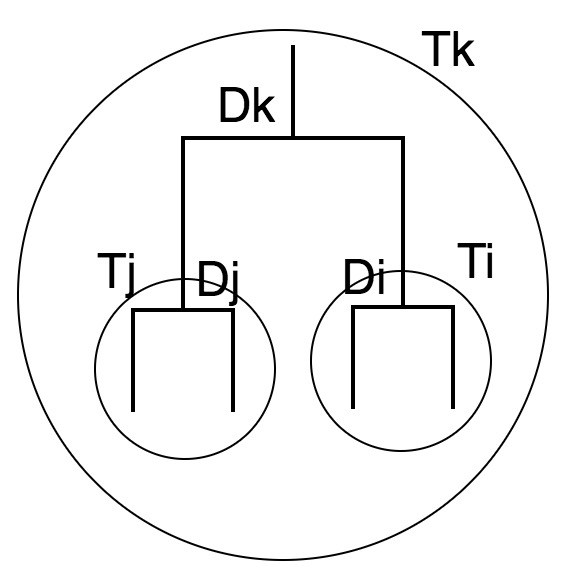
\includegraphics[width=55mm]{figure1.jpeg}
\caption{Schematic of a portion of a tree where $T_i$ and $T_j$ are merged into $T_k$, and associated data sets $D_i$ and $D_j$ are merged into $D_k$} \label{fig1}
\end{figure}

In this paper we reorder the appearance of materials in the original paper. We first introduce Dirichlet Process Mixture Model so that our algorithm raised later is based on this probabilistic model. Then in section 3 we describe the algorithm in detail and give the implementation pseudo code in python. In section 4 we use simulated data and real world data to compare BHC and traditional hierarchical clustering. 

\subsubsection{Notations}
\begin{itemize}
\item $\mathcal{D}:1,\ldots,n$ \ entire data set
\item $T_i:1,\ldots,n$ \ n trivial tree
\item $\mathcal{D}_k:$ \ set of data points at the leaves of subtree $T_k$
\item $\mathcal{H}_1^k:$ \ hypothesis that all the data from the same model
\item $r_k:$ \ the highest probability of the merged hypothesis
\item $\pi_k:$ \ probability of first hypothesis
\item $p(\mathcal{D}_k|T_k):$ \ marginal probability of the data in tree tree $T_k$
\item $\alpha:$ \ learning hyperparameter
\item $C:$ \ number of mixture components
\end{itemize}

\section{Dirichlet Process Mixture Model}
This section follows Rasmuseen(2000)\cite{Ras}. For each of $n$ data points being modelled by a finite mixture, we can associate indicator variables $c_1...c_n$ which can take on values $c_i\in\{1...C\}$ is the number of mixture components. The joint distribution of the indicator variables is multinomial:
$$p(c_1...c_n|\textbf{p})=\prod_{i=1}^C p_k^{n_j},\ n_j=\sum_{i=1}^n \delta(c_i,j)$$

Here $n_j$ is the number of data points assigned to class $j$. As we know that Dirichlet distribution is the conjugate prior distribution of multinomial data, if we place a symmetric Dirichlet prior on \textbf{p} with concentration parameter $\frac{C}{\alpha}$:

$$p(p_1...p_C|\alpha)=\frac{\Gamma(\alpha)}{\Gamma(\alpha/C)^C}\prod_{i=1}^C p_j^{\alpha/C-1}$$

we can integrate \textbf{p} out, obtaining:

\begin{align}
p(c_1...c_n|\alpha)&=\int p(c_1...c_n|p_1...p_C)p(p_1...p_C)dp_1...p_c\\
&=\frac{\Gamma(\alpha)}{\Gamma(\alpha+n)}\prod_{j=1}^C  \frac{\Gamma(n_j+\alpha/C)}{\Gamma(\alpha/C)}
\end{align}

From this we can compute the conditional probability of single indicator:
$$p(c_i=j|\textbf{c}_{-i},\alpha)=\frac{n_{-i,j}+\alpha/C}{n-1+\alpha}$$

where $n_{-i,j}$ is the number of data points, excluding point i, assigned to class j. Finally, taking the infinite limit $(C\rightarrow \infty)$, we obtain:
$$p(c_i=j|\textbf{c}_{-i},\alpha)=\frac{n_{-i,j}}{n-1+\alpha}$$
$$p(c_i\neq c_{i^{'}}\forall i^{'}\neq i |\textbf{c}_{-i},\alpha)=\frac{\alpha}{n-1+\alpha}$$

The second term is the prior probability that point i belongs to some new class that no other points belong to.

Then we give equations for the marginal likelihoods of single components using simple distribution and their conjugate priors. For each component model we compute:

$$p(\mathcal{D}|\mathcal{H}_1)=\int p(\mathcal{D}\theta)p(\theta|\beta)d\theta$$

For Multinomial-Dirichlet conjugate set, we have:

$$p(\mathcal{D}|\mathcal{H}_1)=\prod_{i=1}^N {M_i \choose x_1^{(i)}...x_k^{(i)}}\frac{\Gamma(\sum_{d=1}^k\alpha_d)\prod_{d=1}^k \Gamma(\alpha_d+m_d)}{\Gamma(M+\sum_{d=1}^k\alpha_d)\prod_{d=1}^k \Gamma(\alpha_d)}$$

Other conjugate sets like Bernoulli-Beta and Normal-Inverse Wishart-Normal are also mentioned in the appendix of paper. In our implementation, we follow the main part of the paper. Here derived $p(\mathcal{D}|\mathcal{H}_1)$ is used to calculate $p(\mathcal{D}|T_k)$ and $r_k$, which will be explained in the next section.

\section{BHC Algorithm}

Let $\mathcal{D}$ denote the entire data set, and $D_i\subset \mathcal{D}$ the set of data points at the leaves of the subtree $T_i$. The algorithm is initialized with $n$ single data point $\mathcal{D}_i=\{\textbf{x}^{(i)}\}$. At each stage the algorithm considers merging all pairs of existing trees. 

In considering each merge, two hypothesis are compared. The first hypothesis, which we will denote $\mathcal{H}_1^k$ is that all the data in $\mathcal{D}_k$ were in fact generated from the same probabilistic model(Here we follow DPM). The alternative hypothesis to $\mathcal{H}_1^k$ is that the data in $\mathcal{D}_k$ has two or more cluster. The probability of the data under restricted alternative hypothesis,$\mathcal{H}_2^k$, is simply:
$$p(\mathcal{D}_k|\mathcal{H}_2^k)=p(\mathcal{D}_i|T_i)p(\mathcal{D}_j|T_j)$$

In previous section, we have already computed the probability of the data $\mathcal{D}_k$ under $\mathcal{H}_1^k$, namely $p(\mathcal{D}_k|\mathcal{H}_1^k)$. Combine two probabilities, weighted by the prior that all points in $\mathcal{D}_k$ belong to one cluster,$\pi_k=:p(\mathcal{H}_1^k)$. Then we can get  the marginal probability of the data in tree $T_k$:

$$p(\mathcal{D}_k|T_k)=\pi_k p(\mathcal{D}_k|\mathcal{H}_1^k)+(1-\pi_k)p(\mathcal{D}_i|T_i)p(\mathcal{D}_j|T_j)$$

Under bottom-up DPM model, the posterior probability of the merged hypothesis $r_k=:p(\mathcal{H}_1^k|\mathcal{D}_k)$ is obtained using Bayes rule:

$$r_k=\frac{\pi_k p(\mathcal{D}_k|\mathcal{H}_1^k)}{p(\mathcal{D}_k|\mathcal{H}_1^k)+(1-\pi_k)p(\mathcal{D}_i|T_i)p(\mathcal{D}_j|T_j)}$$

So in each pair of data set we need to find the highest probability of the merged hypothesis $r_k$ to decide which two data sets shall be merge in this turn. The BHC algorithm is very simple:

\begin{algorithm}[H]
    \SetKwInOut{Input}{Input}
    \SetKwInOut{Output}{Output}

    \Input{data $\mathcal{D}=\{x^{(1)}...x^{(n)}\}$, model $p(x|\theta)$, prior $p(\theta|\beta)$ (Here we use DPM)}
    \textbf{Initialization:}{ number of clusters $c=n$, and $\mathcal{D}_i=\{x^{(i)}\}$ for $i=1...n$}\\

    \While{$c>1$}{
    Find the pair $\mathcal{D}_i$ and $\mathcal{D}_j$ with the highest probability of the merged hypothesis:\\
    $r_k=\frac{\pi_k p(\mathcal{D}_k|\mathcal{H}_1^k)}{p(\mathcal{D}_k|T_k)}$
    \;
    Merge $\mathcal{D}_k\leftarrow \mathcal{D}_i \cup \mathcal{D}_j$, $T_k \leftarrow (T_i,T_j)$\;
    Delete $\mathcal{D}_i$ and $\mathcal{D}_j$, $c\leftarrow c-1$\;
    }
    \Output{Bayesian mixture model where each tree node is a mixture component}
    
    The tree can be cut at points where $r_k<0.5$
    \caption{Bayesian Hierarchical Clustering}
\end{algorithm}

\section{Applications to Simulated Data and Real Data}

\subsection{Simulated Data}
In this paper, the authors uses large part to describe the Dirichlet Process mixture model. So int his part, we use Dirichlet distribution to generate 3 different clusters of data with different parameter $\alpha=0.1,0.5,0.9$. Then we use our designed algorithm to cluster this simulated data. The process of merging cluster is as follow:

\begin{figure}
\centering
\includegraphics[width=55mm]{Simulated_data_process.jpeg}
\caption{The process of merging the cluster each time we record the small index} \label{fig2}
\end{figure}

There is no current function to plot mynode, the tree structure which we have defined in our own way. So we have defined a function to plot the tree in the package, so we can use it to plot the leaf nodes and internal nodes in the tree.

\begin{figure}
\centering
\includegraphics[width=55mm]{Simulated_data_tree.jpeg}
\caption{The final tree structure defined by ourselves} \label{fig3}
\end{figure}

And we also plot the distribution of the data. Because the Dirichlet distribution need $\sum x_i=1$, so the point lies on one line $x+y=1$. The plot is as follow:

\begin{figure}
\centering
\includegraphics[width=55mm]{Simulated_data_plot.png}
\caption{The distribution of Dirichlet Data with different parameter} \label{fig4}
\end{figure}

From the process record, tree structure plot, we can see that if we finally tune the tree to make the data fall into three clusters. The result is exactly the same as the simulated process. So the BHC algorithm works well. And we also wonder whether it is comparative to traditional clustering methods. We will do this part in next section.

\subsection{Real Data From Paper}
One real data in the paper is the handwriting data of three numbers:0, 2, 4. So the final class needs to be three. This data contains 120 rows, and 64 columns. Because here we choose DPM model, so we need to pre-process the data to divide each row by its sum so as to keep its sum equal one. And because the limitation of the computation, here we sample 25\% data points from each group. Then we implement our algorithm on the data:

\begin{figure}[htpb]
\centering
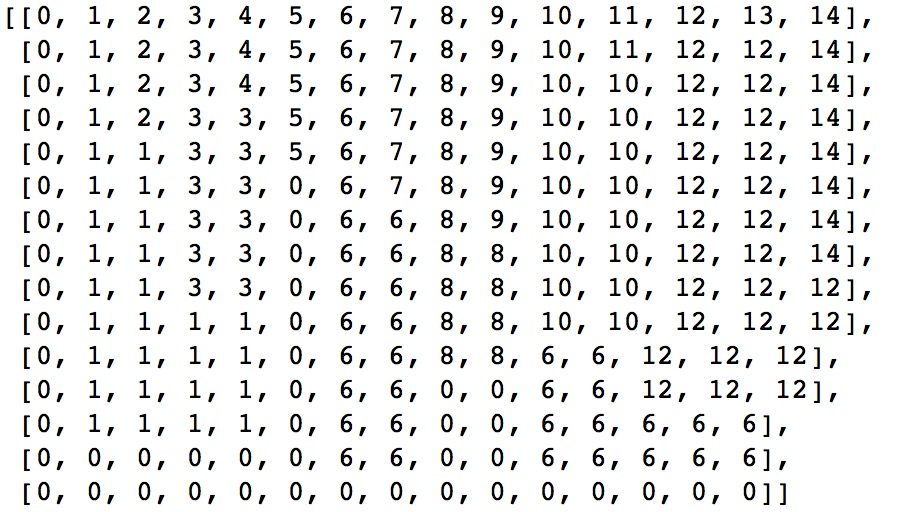
\includegraphics[width=60mm]{toy_example_process.jpeg}
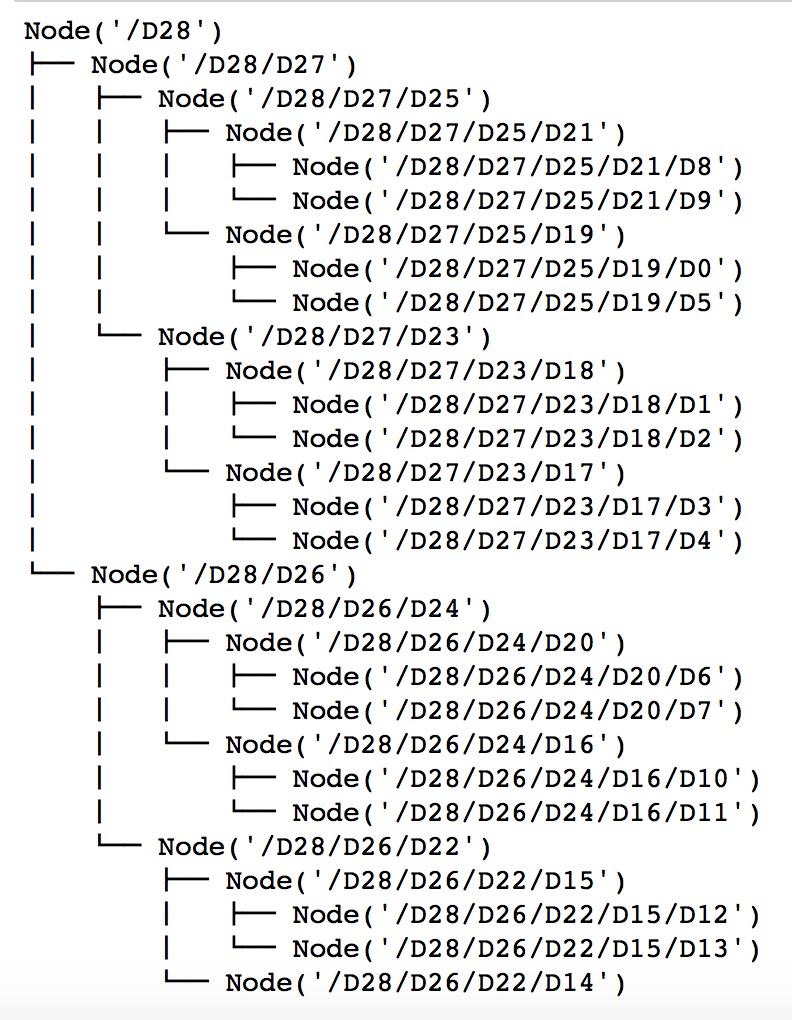
\includegraphics[width=60mm]{toy_example_tree.jpeg}
\caption{The merge process and the final tree structure} 
\label{fig5}
\end{figure}

\subsection{Real Data Not In Paper}
In this part, we use iris data to do clustering. This is perhaps the best known database to be found in the pattern recognition literature. Fisher's paper is a classic in the field and is referenced frequently to this day. The data set contains 3 classes of 50 instances each, where each class refers to a type of iris plant. One class is linearly separable from the other 2; the latter are NOT linearly separable from each other. The final tree structure is like:

From the cluster result, we can find that we can divide birds into three species. But there is a little bias in the prediction. We think this is because the data set is large, and Bayesian Hierarchical Clustering algorithm does not work well when the sample size is large. And here the number of variables is 4. If we apply Bayesian Hierarchical Clustering algorithm to big data area, it will also have problem when calculating the likelihood function and update the highest posterior distribution.

\begin{figure}[htpb]
\centering
\includegraphics[width=55mm]{Iris_data.png}
\caption{The merge process and the final tree structure} 
\label{fig6}
\end{figure}

\section{Comparison to Traditional Hierarchical Clustering}
In this part we implement traditional hierarchical clustering methods on simulated data. And we compare traditional hierarchical clustering methods using three different kinds of linkage. According to different definitions of distance, we have single linkage, complete linkage and average linkage. Single linkage uses the shortest distance of two points between two groups to measure similarity. Complete linkage uses the shortest distance of two points between two groups. And average linkage uses the average distance of all points in two groups.

The final dendrograms are as follow:

\begin{figure}[h]
\centering
\subfigure[SingleLinkage]{
\includegraphics[width=50mm]{SingleLinkage.png}
}
\subfigure[CompleteLinkage]{
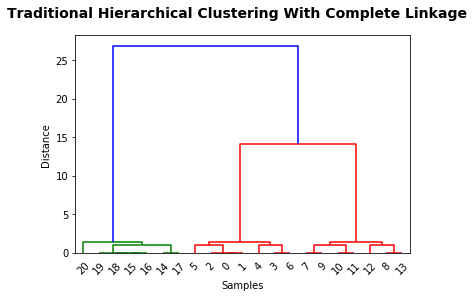
\includegraphics[width=50mm]{CompleteLinkage.png}
}
\subfigure[AverageLinkage]{
\includegraphics[width=50mm]{AverageLinkage.png}
}
\caption{Traditional Hierarchical Clustering With Different Linkage}
\label{fig:THC}
\end{figure}

According to the dendrograms below, the dendrogram by using single linkage is most similar to what we do for the BHC model. Especially, the complete linkage and the average linkage have the same result.  

In this part we did not use Hierarchical Clustering to compare with k-means method. Both methods have their own advantages and disadvantages. It's a reminder that if we know how many categories data will fall into, then k-means may perform better. 

\section{Profiling and Optimization}

\subsection{Profiling Difficulty of Implementation}
BHC algorithm needs to calculate the likelihood function. In python, when calculating large factorial number, it may cause overflow problem. So we use loggamma function to replace gamma function to make it small so that it can do basic calculations.

Secondly, it is hard to represent a node in python. There is no current class for the BHC algorithm. After referring to the tree class, we define a new class called mynode in python to implement the algorithm. In mynode class, there are 7 attributes: left, right, data, cluster, alpha, index , parent. Defining such a class makes the implementation handy to carry on.

Thirdly, if the data set does not follow a Dirichlet distribution, we need to change the model to compute $p(\mathcal{D}_k|\mathcal{H}_1^k)$. And it is common that when the sample size is large using any agglomerative hierarchical clustering method will have large computational cost.  So we use jit and other optimization method to speed up our code.

\subsection{Optimization}

\subsubsection{Naive Version:}

For the Bayesian hierarchical clustering, we wrote our algorithm in numpy for most parts. We define one python class mynode, one main function bhc, and six small functions. 

\begin{figure}[htpb]
\centering
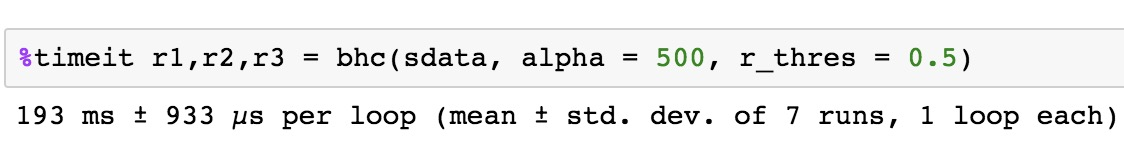
\includegraphics[width=90mm]{r4.jpeg}
\caption{The time naive code costs} 
\label{fig8}
\end{figure}

In our original code, there are a lot places needed to be improved. From the result, we know that we can optimize the code because there are some for loops to find the highest posterior merge probability. In the following, we use several methods to improve the speed.

\subsubsection{Merging Small Function:} In our algorithm, we need to calculate $d_k$, $r_k$, and $\pi_k$. In the algorithm shown in the original paper, the author list these values respectively. But we can calculate these values in one function so that it might save time. 

In the original paper, the author provides a recursive function to compute each value. In mathematics, it is easy to understand. But it will increase the computational cost. Here we store the value of internal nodes, so that we do not to trace back to the leaf nodes. Although this will need more memory, we believe this will save time at the same.

\begin{figure}[htpb]
\centering
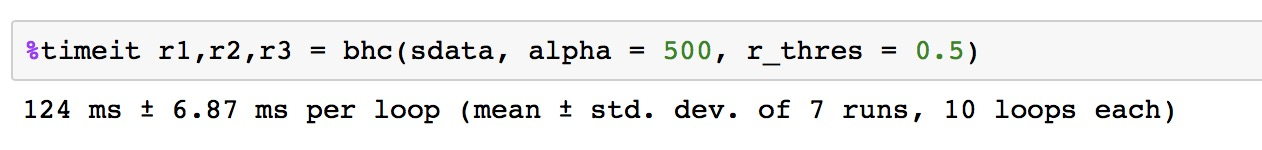
\includegraphics[width=90mm]{r3.jpeg}
\caption{The time Merging Small Function costs} 
\label{fig9}
\end{figure}

\subsubsection{Using Numby vectorized:}

In our algorithm, all the calculation can be done in the multiplication of array. So we use Numby vectorized to optimize the code.

\begin{figure}[htpb]
\centering
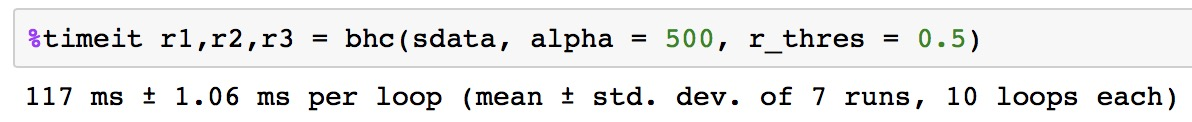
\includegraphics[width=90mm]{r1.jpeg}
\caption{The time Numby vectorized costs} 
\label{fig10}
\end{figure}

\subsubsection{Using jit nopython:}
Here we try @jit and nopython= None to optimize the code in another way. but it shows that there is little difference between this one and the previous one. 

\begin{figure}[h]
\centering
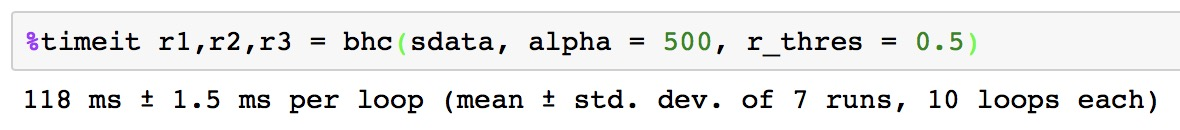
\includegraphics[width=90mm]{r2.jpeg}
\caption{The time Merging Small Function costs} 
\label{fig11}
\end{figure}

And we have also tried iparallel, cython methods. But because here we define a new class mynode, it's hard to specify the input class through cython. And we also search a lot of references, maybe this is still a problem in the speed of hierarchical clustering.

\section{Limitation and Further Improvement}
As mentioned before, the calculation of likelihood function may cause overflow problem if not using the log gamma function. And when the data set and the prior are not conjugate, there is no closed form of the likelihood function. And also it is a common problem for agglomerative hierarchical algorithm that it is much slower than other clustering like k-means method when the sample size is large.

The initialization process of choosing the two initial points need to be more automatic. The only algorithm I can think of currently is the greedy algorithm that choose the 2 initial points pairwise, like the traditional hierarchical clustering algorithm does.
When the sample size is larger than 100, there is possible an integration error;
make the algorithm to accomodate the multinomial distribution;
withough given the exact number of clusters the data are from, the algorithm can learn the number of clusters the data from through the iteraion;
Without given the conjugate distribution, the algorithm can find the optimal likelihood through the EM optimization.

\section{Conclusion}
BHC has more advantages over the traditional algorithm. BHC defines a probabilistic model of the data which can be used to computed the predictive distribution. And the traditional Agglomerative Hierarchical Algorithm has limitations: there is no certain rubric to decide the number of clusters to choose. The nearest pair of clusters is chosen based on a given distance measure. As discussed before, we can use single linkage, complete linkage and average linkage. It's hard to evaluate whether the model is good or bad.

However, the BHC model also has its shortage. The likelihood function is not easy to compute and may cause overflow problem which have been illustrated in the profiling section. This requires a high computation complexity and make algorithm run slowly.

\begin{thebibliography}{8}
\bibitem{ref_article1}
Heller, Katherine A., and Zoubin Ghahramani. "Bayesian Hierarchical Clustering." Proceedings of the 22nd International Conference on Machine Learning - ICML '05, 2005, doi:10.1145/1102351.1102389.

\bibitem{Ras}
Rasmussen, C. F. (2000). The infinite Gaussian mixture model. NIPS 12 (pp. 554--560).

\bibitem{DPM}
Blei, D., Jordan, M. (2004). Variational methods for dirichlet process mixture models (Technical Report 674). UC Berkeley.

\bibitem{DPMM}
 Vasilis Vryniotis (2014). 
The Dirichlet Process Mixture Model. \url{http://blog.datumbox.com/the-dirichlet-process-mixture-model/}


\end{thebibliography}
\end{document}
\end{align*}
\end{document}